\chapter{Επίλογος}
Στο τελευταίο κεφάλαιο, πραγματοποιείται συνοπτική παρουσίαση των θεμάτων που αναλύθηκαν έως τώρα. Στη συνέχεια παρουσιάζονται τα συμπεράσματα που προέκυψαν κατά τη διαδικασία σχεδίασης και κατασκευής της διαδικτυακής εφαρμογής.
Επιπλέον, γίνεται λεπτομερής ανάλυση SWOT (Strengths, Weaknesses, Opportunities, Threats) του συστήματος, καθώς και προτάσεις για μελλοντικές βελτιστοποιήσεις και επεκτάσεις των λειτουργιών που παρέχει.

\section{Ανακεφαλαίωση Διπλωματικής Εργασίας}
Οι ανάγκες δικτυακής εκκίνησης υπολογιστών του Εργαστηρίου Ρομποτικής, Ενσωματωμένων και Ολοκληρωμένων Συστημάτων του Πανεπιστημίου Δυτικής Μακεδονίας, απαιτούσαν μια διαδικτυακή εφαρμογή με συγκεκριμένα χαρακτηριστικά και δυνατότητες που δεν ήταν διαθέσιμες σε εμπορικές λύσεις. Για την κάλυψη αυτών των αναγκών, αναπτύχθηκε η διαδικτυακή εφαρμογή `iBoot'.

Η εφαρμογή `iBoot' αναπτύχθηκε χρησιμοποιώντας PHP στο back-end και HTML, CSS, JavaScript και Bootstrap στο front-end. Τα δεδομένα της εφαρμογής αποθηκεύονται σε μια σχεσιακή βάση δεδομένων MySQL. Η πρόσβαση στην εφαρμογή μπορεί να γίνει είτε μέσω μιας διεπαφής χρήστη είτε μέσω ενός REST API που αναπτύχθηκε για αυτόν το σκοπό. Ο πηγαίος κώδικας της εφαρμογής είναι δημόσια διαθέσιμος και διαμοιράζεται υπό τους όρους της ελεύθερης άδειας χρήσης λογισμικού MIT.

Η εφαρμογή διευκολύνει την πρόσβαση σε τρεις τύπους χρηστών.
Ένας ανώνυμος χρήστης έχει πρόσβαση μόνο στις σελίδες σύνδεσης, εγγραφής και υπενθύμισης των διαπιστευτηρίων σύνδεσης.
Ο διαχειριστής εργαστηρίου μπορεί να διαχειρίζεται υπολογιστές σε συγκεκριμένα εργαστήρια. Μπορούν επίσης να τοποθετηθούν υπολογιστές σε εργαστήρια που διαχειρίζεται ο διαχειριστής και οι οποίοι δεν έχουν ήδη τοποθετηθεί σε άλλα εργαστήρια.
Ο διαχειριστής μπορεί να χρησιμοποιεί όλες τις δυνατότητες της πλατφόρμας χωρίς περιορισμούς. Ο διαχειριστής έχει την εξουσία να προσθέτει, να αφαιρεί και να τροποποιεί υπολογιστές, ομάδες, εργαστήρια, μπλοκ iPXE, μενού εκκίνησης, χρονοδιαγράμματα και χρήστες. Ο Διαχειριστής επιτρέπεται επίσης να βλέπει τα αρχεία καταγραφής συμβάντων της εφαρμογής.
Οι υπολογιστές επικοινωνούν με συγκεκριμένες σελίδες της εφαρμογής για να εγγραφούν και να λάβουν μενού εκκίνησης.

Η εφαρμογή έχει σχεδιαστεί και υλοποιηθεί σύμφωνα με τις βέλτιστες πρακτικές και τα πιο πρόσφατα πρότυπα ασφαλείας για την προστασία των πληροφοριών που περιέχονται σε αυτήν. Οι κωδικοί πρόσβασης των χρηστών αποθηκεύονται στη βάση δεδομένων της εφαρμογής αφού υποστούν επεξεργασία μέσω κρυπτογραφικά ασφαλών συναρτήσεων κατακερματισμού και δεν εμφανίζονται ποτέ στην εφαρμογή. Η πιστοποίηση ταυτότητας και τα δικαιώματα του χρήστη που επιθυμεί να προβάλει τη σελίδα ελέγχονται πριν από τη φόρτωση, ενώ το API υλοποιεί την ίδια διαδικασία προσθέτοντας σε κάθε αίτηση JWT tokens. Η εφαρμογή είναι σε θέση να λειτουργεί τόσο με το πρωτόκολλο HTTP όσο και με το πιο ασφαλές πρωτόκολλο HTTPS και μπορεί ακόμη και να κρυπτογραφήσει τα cookies συνόδου.

Το Εργαστήριο Ρομποτικής, Ενσωματωμένων και Ολοκληρωμένων Συστημάτων του Πανεπιστημίου Δυτικής Μακεδονίας θα εκσυγχρονίσει τη διαδικασία διαχείρισης του μενού εκκίνησης του δικτύου των υπολογιστών του με την εγκατάσταση της διαδικτυακής εφαρμογής ``iBoot'', η οποία θα διευκολύνει επίσης σημαντικά την καταγραφή και την παρακολούθηση των υπολογιστών αυτών.

\section{Μοντέλο Ανάλυσης S.W.O.T.}

\subsection{Ορισμός Μοντέλου Ανάλυσης S.W.O.T.}
Η ανάλυση SWOT, ή πίνακας SWOT, είναι ένα εργαλείο στρατηγικού σχεδιασμού και διαχείρισης που χρησιμοποιείται για να επιτρέψει σε άτομα ή οργανισμούς να εντοπίσουν τα δυνατά σημεία, τις αδυναμίες, τις ευκαιρίες και τις απειλές που σχετίζονται με τον επιχειρηματικό ανταγωνισμό ή τον προγραμματισμό έργων.

Η τεχνική αυτή προορίζεται για χρήση κατά τα προκαταρκτικά στάδια των διαδικασιών λήψης αποφάσεων για την αξιολόγηση της στρατηγικής θέσης. Σκοπός της είναι να εντοπίσει τόσο εσωτερικούς όσο και εξωτερικούς παράγοντες που είναι είτε ευνοϊκοί είτε δυσμενείς για την επίτευξη των στόχων του έργου ή της πρωτοβουλίας.

Ο όρος αποτελεί ακρωνύμιο των τεσσάρων στοιχείων τα οποία αξιολογεί η μέθοδος:

\begin{description}
	\item[Δυνάμεις:] χαρακτηριστικά της επιχείρησης ή του έργου που παρέχουν πλεονέκτημα έναντι του ανταγωνισμού
	\item[Αδυναμίες:] χαρακτηριστικά που θέτουν την επιχείρηση ή το έργο σε μειονεκτική θέση σε σχέση με τον ανταγωνισμό
	\item[Ευκαιρίες:] παράγοντες του περιβάλλοντος που μπορεί να εκμεταλλευτεί η επιχείρηση ή το έργο
	\item[Απειλές:] παράγοντες του περιβάλλοντος που θα μπορούσαν να αποτελέσουν προκλήσεις για την επιχείρηση ή το έργο
\end{description}

Τα αποτελέσματα της αξιολόγησης εμφανίζονται συνήθως είτε σε μορφή πίνακα είτε σε παραγράφους.

\subsubsection{Εσωτερικοί - Εξωτερικοί Παράγοντες}
Οι εσωτερικές πτυχές μιας επιχείρησης θεωρούνται συνήθως ως πλεονεκτήματα ή αδυναμίες, ενώ οι ευκαιρίες ή οι απειλές θεωρούνται ως εξωτερικές.

Οι εσωτερικοί παράγοντες ενός οργανισμού αξιολογούνται ως πλεονεκτήματα ή αδυναμίες, με βάση τον αντίκτυπό τους στους στόχους της επιχείρησης. Κάτι που θα μπορούσε να θεωρηθεί ως πλεονέκτημα για έναν στόχο μπορεί να θεωρηθεί ως αδυναμία για έναν άλλο, για παράδειγμα, ο ανταγωνισμός ή οι περισπασμοί. Οι παράγοντες μπορεί να περιλαμβάνουν το προσωπικό, τη χρηματοδότηση, τις δυνατότητες παραγωγής και όλα τα 4P του μείγματος μάρκετινγκ (προϊόν, τιμή, θέση και προώθηση).

Οι εξωτερικοί παράγοντες περιέχουν κοινωνικοπολιτισμικές αλλαγές, μακροοικονομικές εξελίξεις, νομοθετικές εξελίξεις, τεχνολογικές εξελίξεις, καθώς και μετατοπίσεις στην αγορά.

\subsection{Ανάλυση S.W.O.T. εφαρμογής iBoot}
Στο σχήμα \ref{fig:iBoot_swot_analysis} απεικονίζεται η ανάλυση S.W.O.T. της διαδικτυακής εφαρμογής iBoot. Τα ευρήματα της ανάλυσης αναλύονται στη συνέχεια, το καθένα στην αντίστοιχη υποενότητα.

\begin{figure}[ht]
	\centering
	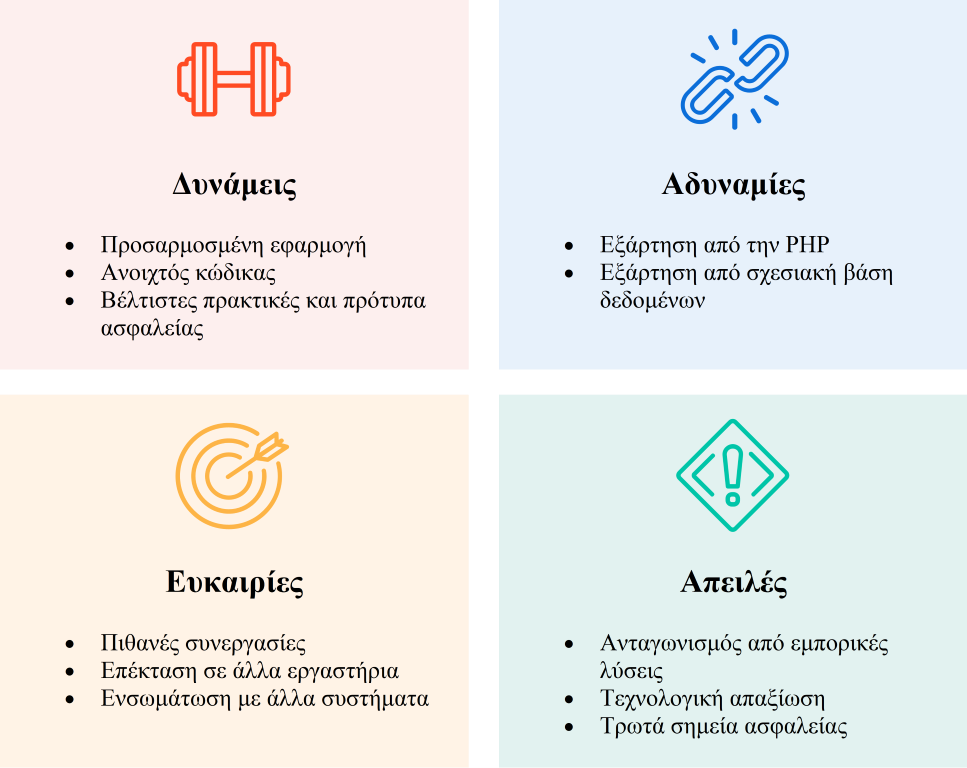
\includegraphics[scale=0.5]{swot-analysis.png}
	\caption{Ανάλυση SWOT εφαρμογής iBoot}
	\label{fig:iBoot_swot_analysis}
\end{figure}

\subsubsection{Δυνάμεις}
\begin{description}
	\item[Προσαρμοσμένη εφαρμογή:] Η εφαρμογή iBoot αναπτύχθηκε ειδικά για να ανταποκρίνεται στις απαιτήσεις του Εργαστηρίου Ρομποτικής, Ενσωματωμένων και Ολοκληρωμένων Συστημάτων, διασφαλίζοντας ότι διαθέτει τα απαραίτητα χαρακτηριστικά και δυνατότητες.
	\item[Ανοιχτός κώδικας:] Ο πηγαίος κώδικας της εφαρμογής είναι διαθέσιμος στο κοινό και δημοσιεύεται με την άδεια MIT, επιτρέποντας τη διαφάνεια και τις πιθανές συνεισφορές της κοινότητας.
	\item[Βέλτιστες πρακτικές και πρότυπα ασφαλείας:] Η εφαρμογή έχει σχεδιαστεί και υλοποιηθεί σύμφωνα με τις βέλτιστες πρακτικές και τα πιο πρόσφατα πρότυπα ασφαλείας, διασφαλίζοντας την προστασία των πληροφοριών και την κρυπτογράφηση των cookies συνόδου.
\end{description}

\subsubsection{Αδυναμίες}
\begin{description}
	\item[Εξάρτηση από την PHP:] Το back-end της εφαρμογής iBoot είναι κατασκευασμένο με τη χρήση PHP, η οποία μπορεί να δημιουργήσει προκλήσεις όσον αφορά την επεκτασιμότητα και τη συμβατότητα με μελλοντικές τεχνολογίες.
	\item[Εξάρτηση από σχεσιακή βάση δεδομένων:] Η εφαρμογή βασίζεται σε μια σχεσιακή βάση δεδομένων MySQL για την αποθήκευση δεδομένων, γεγονός που ενδέχεται να περιορίσει την επεκτασιμότητα και την απόδοση κατά τον χειρισμό μεγάλων όγκων δεδομένων.
\end{description}

\subsubsection{Ευκαιρίες}
\begin{description}
	\item[Πιθανές συνεργασίες:] Η φύση της εφαρμογής ως ανοικτού κώδικα δημιουργεί ευκαιρίες συνεργασίας με άλλα ιδρύματα ή προγραμματιστές που μπορούν να συμβάλουν στην περαιτέρω βελτίωσή της.
	\item[Επέκταση σε άλλα εργαστήρια:] Η επιτυχία και ο θετικός αντίκτυπος της εφαρμογής iBoot στο Εργαστήριο Ρομποτικής, Ενσωματωμένων και Ολοκληρωμένων Συστημάτων μπορεί να οδηγήσει στην υιοθέτησή της από άλλα εργαστήρια εντός του Πανεπιστημίου Δυτικής Μακεδονίας ή και πέραν αυτού.
	\item[Ενσωμάτωση με άλλα συστήματα:] Η εφαρμογή μπορεί να διερευνήσει ευκαιρίες για ενσωμάτωση με άλλα συστήματα ή πλατφόρμες, επιτρέποντας βελτιωμένη λειτουργικότητα και διαλειτουργικότητα.
\end{description}

\subsubsection{Απειλές}
\begin{description}
	\item[Ανταγωνισμός από εμπορικές λύσεις:] Παρόλο που η εφαρμογή iBoot αναπτύχθηκε για να ικανοποιήσει συγκεκριμένες απαιτήσεις, υπάρχει πιθανότητα ανταγωνισμού από εμπορικές λύσεις που μπορεί να προσφέρουν περισσότερα χαρακτηριστικά ή ευρύτερο φάσμα δυνατοτήτων.
	\item[Τεχνολογική απαξίωση:] Οι ταχείες εξελίξεις στην τεχνολογία ενδέχεται να καταστήσουν ορισμένες πτυχές της εφαρμογής ξεπερασμένες, απαιτώντας συνεχείς ενημερώσεις και προσαρμογές για να παραμείνει επίκαιρη.
	\item[Τρωτά σημεία ασφαλείας:] Παρά την τήρηση των βέλτιστων πρακτικών και των προτύπων ασφαλείας της εφαρμογής, υπάρχει ο κίνδυνος τρωτών σημείων ασφαλείας και πιθανών παραβιάσεων, οι οποίες θα μπορούσαν να θέσουν σε κίνδυνο τις πληροφορίες και τη λειτουργικότητα της εφαρμογής.
\end{description}

\section{Μελλοντικές Επεκτάσεις}
Όλες οι διαδικτυακές εφαρμογές οφείλουν να αναβαθμίζονται συνεχώς ώστε, πέρα από την προσθήκη νέων δυνατοτήτων και τη βελτίωση των υπαρχόντων, να παραμένουν λειτουργικές και ασφαλείς. Συχνά χρειάζεται επίσης και η ενημέρωση βιβλιοθηκών και άλλων εξαρτήσεων της εφαρμογής, ώστε να καλύπτονται πιθανά κενά ασφαλείας και να επιλύονται προβλήματα που ίσως υπάρχουν. Η διαδικτυακή εφαρμογή που αναπτύχθηκε δεν αποτελεί εξαίρεση. Η βιωσιμότητα της είναι άμεσα εξαρτώμενη από τις εργασίες συντήρησης και ενημέρωσης της, οι οποίες θα πρέπει να πραγματοποιούνται τακτικά.

Μερικές ιδέες για περαιτέρω ανάπτυξη της εφαρμογής παρουσιάζονται στη συνέχεια.

\begin{description}
	\item[Διεύρυνση λειτουργιών του REST API:] To REST API θα μπορούσε να διευρυνθεί, προσθέτοντας endpoints που θα προσφέρουν διαλειτουργικότητα με άλλες εφαρμογές και υπηρεσίες. Αν αξιολογηθεί ως σημαντικό, θα μπορούσαν να προστεθούν συναρτήσεις ανάκτησης τμήματος δεδομένων, με περισσότερους ελέγχους πρόσβασης. Τέλος, θα ήταν ίσως χρήσιμη η προσθήκη μιας προαιρετικής παραμέτρου σελιδοποίησης, ώστε να αντλείται συγκεκριμένος αριθμός εγγραφών από την κάθε κλήση στα endpoints του API. Κάτι τέτοιο θα βελτίωνε την απόδοση της εφαρμογής σε μεγάλους αριθμούς εγγραφών.
	\item[Ανάπτυξη εναλλακτικών front-end:] Η ύπαρξη του REST API ευνοεί τη δημιουργία εναλλακτικών front-end για την εφαρμογή, αφού ουσιαστικά το front-end με το back-end είναι αποσυνδεδεμένα και επικοινωνούν μέσω του API της εφαρμογής. Ένα εναλλακτικό front-end θα μπορούσε να προσφέρει μεγαλύτερη συμβατότητα με συγκεκριμένους τύπους συσκευών, να εμφανίζει τις πληροφορίες της εφαρμογής με έναν πιο μοντέρνο και παραμετροποιήσιμο τρόπο, ή ακόμη και να πακεταριστεί σε εγγενή εφαρμογή για κάποιο λειτουργικό σύστημα υπολογιστών.
	\item[Υποστήριξη διαφορετικών μεθόδων αυθεντικοποίησης:] Η εγγραφή και σύνδεση στο σύστημα θα μπορούσε να αξιοποιεί υπάρχοντα πρωτόκολλα διαπιστευτηρίων, ώστε να υποστηρίζεται και η διαλειτουργικότητα με την υπόλοιπη υποδομή κάποιου εργαστηρίου. Τέτοια πρωτόκολλα είναι τα LDAP, OAuth2, SAML και άλλα. Επίσης, θα μπορούσε να αναπτυχθεί υποστήριξη για σύνδεση με χρήση πολλαπλών παραγόντων ή και σύνδεσης χωρίς κωδικό πρόσβασης με magic link στο email του χρήστη.
	\item[Προσθήκη λειτουργίας Wake-on-Lan:] Θα μπορούσε να διερευνηθεί η δυνατότητα δημιουργίας και αποστολής Wake-on-Lan πακέτων στο δίκτυο των υπολογιστών, ώστε η διαδικασία εκκίνησής τους να μπορεί να ξεκινήσει απευθείας από την εφαρμογή και χωρίς φυσική πρόσβαση στο κάθε μηχάνημα.
	\item[Τροποποίηση ημερολογίου σε επεξεργάσιμο:] Το ημερολόγιο των χρονοδιαγραμμάτων θα μπορούσε να γίνει επεξεργάσιμο και έτσι δημιουργία νέων  ή η τροποποίηση υπαρχόντων χρονοδιαγραμμάτων να γίνεται απευθείας σε αυτό.
	\item[Προσθήκη δυνατότητας ανακατάταξης των Μπλοκ iPXE:] Θα μπορούσε να προστεθεί η δυνατότητα ανακατάταξης των Μπλοκ iPXE μέσα σε κάθε μενού, ώστε ο χρήστης να μπορεί να αλλάξει τη σειρά με την οποία εμφανίζονται κατά την εκκίνηση υπολογιστών, αντί για την μη-παραμετροποιήσιμη σειρά απεικόνισης που υπάρχει τώρα, καταταγμένη βάση της χρονολογικής σειράς με την οποία προστέθηκαν τα Μπλοκς στο κάθε μενού.
	\item[Ενσωμάτωση relay DHCP server:] Η εφαρμογή θα μπορούσε να ενσωματώσει έναν relay DHCP server, ώστε να μπορεί να εγκατασταθεί στο τοπικό δίκτυο και να λειτουργήσει χωρίς επεξεργασία των ρυθμίσεων του προϋπάρχοντος DHCP server του δικτύου.
\end{description}

\section{Συμπεράσματα}
Από την παρούσα διπλωματική εργασία μπορεί να προκύψει μια πληθώρα συμπερασμάτων, σχετικά είτε με τις διαδικτυακές εφαρμογές γενικότερα, είτε ειδικότερα για τη συγκεκριμένη εφαρμογή διαχείρισης δικτυακής εκκίνησης υπολογιστών που αναπτύχθηκε.

Αρχικά, έγινε ανάλυση του διαδικτύου και τον ρόλο των εφαρμογών του στη σύγχρονη εποχή. Επίσης, έγινε αναφορά σε διάφορες γλώσσες διαδικτυακού προγραμματισμού, αλλά και τεχνικές οι οποίες αποσκοπούν να διευκολύνουν και να επιταχύνουν την ανάπτυξη εφαρμογών και να τις καταστήσουν πιο συντηρήσιμες και ασφάλειες. Μπορούμε από τα παραπάνω να συμπεράνουμε, ότι παρά την ταχεία τεχνολογική εξέλιξη, και την πληθώρα τεχνικών και εργαλείων που συνεχώς βελτιώνονται και αλλάζουν, η σημασία των διαδικτυακών εφαρμογών ως μέσων επίλυσης πρακτικών προβλημάτων παραμένει αναλλοίωτη σε βάθος χρόνου. Αυτό κάνει και σημαντικό προσόν την τεχνογνωσία σχεδίασης, ανάπτυξης και συντήρησής τους.

Στη συνέχεια, αναλύθηκαν η σχεδίαση και υλοποίηση της διαδικτυακής εφαρμογής δικτυακής εκκίνησης υπολογιστών iBoot. Γινεται εύκολα εμφανές, ότι για την επιτυχημένη ανάπτυξη μιας εφαρμογής, πρέπει να έχει γίνει αναλυτική σχεδίαση των δεδομένων που θα μεταχειρίζεται, των λειτουργιών της και του τρόπου απεικόνισής της. Φυσικά, για τη σχεδίαση της λύσης, πρέπει να έχει προηγηθεί μια καλή ανάλυση του προβλήματος προς επίλυση. Συμπεράνουμε δηλαδή, πώς η σωστή ακολουθία φάσεων ανάπτυξης μιας εφαρμογής, της οποίας βήματα δε πρέπει να παραλείπονται ή να παραβλέπονται, είναι:
\begin{enumerate}
	\item Διεξοδική ανάλυση του προβλήματος.
	\item Καθορισμός προδιαγραφών και σχεδιασμός λύσης.
	\item Ανάπτυξη λύσης, βάση των ορισμένων προδιαγραφών.
	\item Έλεγχος ποιότητας λύσης και ανατροφοδότηση.
\end{enumerate}

Επιπρόσθετα, έγινε αξιολόγηση του συστήματος που παράχθηκε, με γνώμονα τόσο την ποιότητα και τη χρησιμότητα της λύσης που προσφέρει, όσο και τη βιωσιμότητα του, καθώς και την ικανότητα του να κλιμακωθεί, ώστε να σε αυξημένες ανάγκες. Από αυτό, μπορούμε να αντλήσουμε το συμπέρασμα πως, όπως αναφέρθηκε και παραπάνω, αν και συμβαίνουν στην τελευταία φάση του κύκλου ζωής ανάπτυξης μιας εφαρμογής, ο έλεγχος της και η ανατροφοδότηση είναι ιδιαίτερα σημαντικά. Σε αυτή τη φάση αξιολογείται, ουσιαστικά, αν η εφαρμογή πέτυχε το σκοπό για τον οποίο δημιουργήθηκε, αν είναι ασφαλής και σταθερή, και πώς μπορεί να βελτιωθεί περαιτέρω.

Τέλος, όσον αφορά τη συγκεκριμένη εφαρμογή, μπορούμε να συμπεράνουμε πως η διαδικασία διαχείρισης δικτυακής εκκίνησης υπολογιστών για ένα πανεπιστημιακό εργαστήριο, μπορεί να γίνει αρκετά περίπλοκη σε βάθος χρόνου και καθώς αυξάνονται οι απαιτήσεις. Η χρήση της εφαρμογής θα έχει σημαντικό όφελος για το εργαστήριο, αφού θα απλοποιήσει τη διαδικασία και θα αποδεσμεύσει πολύτιμο χρόνο των διαχειριστών, οι οποίοι θα μπορούν πλέον να προβάλλουν και να τροποποιούν πολύ εύκολα τα χρονοδιαγράμματα εκκίνησης των υπολογιστών του εργαστηρίου.

\section{Σύνοψη Κεφαλαίου 6}
Το κεφάλαιο 6 σηματοδοτεί το πέρας της παρούσας διπλωματικής εργασίας. Στο παρόν κεφάλαιο παρέχεται μια ανάλυση SWOT του περιεχομένου της διαδικτυακής πλατφόρμας, η οποία περιγράφει συνοπτικά τα πλεονεκτήματα και τα μειονεκτήματα που σχετίζονται με την υλοποίηση του παρόντος έργου, καθώς και τις δυνατότητες και τα οφέλη που παρουσιάζει και τυχόν πιθανούς κινδύνους που μπορεί να αντιμετωπίσει. Παρέχονται επίσης ορισμένες ιδέες για πιθανές μελλοντικές βελτιώσεις και προσαρμογές της πλατφόρμας. Το κεφάλαιο αυτό ολοκληρώνεται με τα τελικά συμπεράσματα επί της διπλωματικής εργασίας.
